\documentclass{beamer}

\usepackage[utf8x]{inputenc}
\usepackage{default}

\usepackage{amsmath}

\usepackage{multicol}
\usepackage{url}
\usepackage{graphicx}

%figures
%\usepackage{wrapfig}

%font
\usepackage[T1]{fontenc}
\usepackage{venturis}

\usecolortheme{beaver}

%titlepage
\title{Simulation of the unstable rotation of a cuboid}
\subtitle{Books in space}
\author{Ivar Postma \and Eamon Nerbonne}
\institute[University of Groningen]
{
  Introduction to Computational Science \\
  School for Computing and Cognition \\
  University of Groningen
}
\date{December 1, 2011}

\begin{document}

\frame{\titlepage}

\begin{frame}
 \frametitle{Experiment in space}
 \begin{figure}
  \centering
  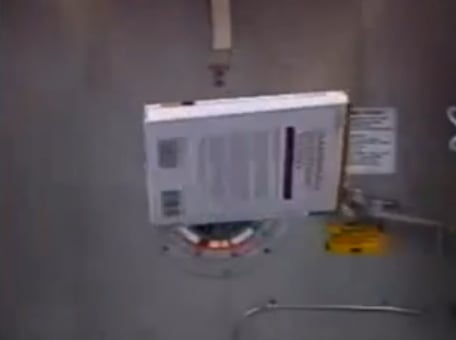
\includegraphics[width=0.4\textwidth]{book.png}
 \end{figure}


 \begin{itemize}
  \item \url{http://www.youtube.com/watch?v=GgVpOorcKqc}
 \end{itemize}
\end{frame}

\begin{frame}
 \frametitle{Stable and unstable rotation}
 \begin{itemize}
  \item The book can stably rotate around two of its axis
  \item Rotation around the third axis is not stable
 \end{itemize}
\end{frame}

\begin{frame}
 \frametitle{Modelling the behaviour}
 We make a few simplifications
 \begin{itemize}
  \item The book is a cuboid
  \item The density is constant
 \end{itemize}
\end{frame}

\begin{frame}
 \frametitle{Model}
 \framesubtitle{State vector}
 For a point on the body we keep track of the position, the orientation, the total linear momentum and the total angular momentum

 \begin{displaymath}
  S(t) = \begin{pmatrix}
          x(t) \\
	  R(t) \\
	  P(t) \\
	  L(t)
         \end{pmatrix}
 \end{displaymath}
\end{frame}

\begin{frame}
 \frametitle{Model}
 \framesubtitle{Updating the sate vector}
 To update we need the velocity, the angular speed, the force and the torque (moment of force)

 \begin{displaymath}
  \frac{d}{dt} S(t) = \begin{pmatrix}
          v(t) \\
	  \omega(t) * R(t) \\
	  F(t) \\
	  \tau(t)
         \end{pmatrix}
 \end{displaymath}
\end{frame}

\begin{frame}
 \frametitle{Model}
 \framesubtitle{More simplifications}
 When a book is rotating in space, the model is simple because
 \begin{itemize}
  \item there is no force, $F(t) = 0$
  \item there is no torque, $\tau(t) = 0$
 \end{itemize}
 Thus, we only need to calculate the velocity and angular speed
\end{frame}

\begin{frame}
 \frametitle{Model}
 \framesubtitle{Updating the state vector}
 Velocity is given by
 \begin{displaymath}
  v(t) = \omega(t) r(t)
 \end{displaymath}
 
 Angular speed is given by
 \begin{displaymath}
  \omega(t) = I(t)^{-1} L(t)
 \end{displaymath}

 $I(t)$ depends on $R(t)$ and the moment of inertia of the body $I_{body}$
 \begin{displaymath}
  I(t) = R(t) I_{body} R(t)^{T}
 \end{displaymath}
\end{frame}

\begin{frame}
 \frametitle{Moment of inertia}
 \begin{itemize}
  \item 
  The moment of inertia of an object is a measure of the resistance of an object to changes in the rotation

  \item
  For a cuboid the moment of inertia is given by
  \begin{displaymath}
    I_{body} = \frac{1}{12} \begin{pmatrix}
			    M(b^2 + c^2) & 0 & 0 \\
			    0 & M(a^2 + c^2) & 0 \\
			    0 & 0 & M(a^2 + b^2)
			    \end{pmatrix}
  \end{displaymath}
  where $a, b$ and $c$ are the dimensions of the cuboid
 \end{itemize}
\end{frame}

\begin{frame}
 \frametitle{Methods to solve the calculations}
 \begin{itemize}
  \item Euler intergration
  \item Midpoint method
  \item 4th order Runga Kutta
 \end{itemize}
\end{frame}

\begin{frame}
 \frametitle{Implementation}
 We intend to implement this in C/C++ using OpenGL for the visualisation
\end{frame}

 \begin{frame}
  \frametitle{Questions?}
 \end{frame}


\end{document}
